\documentclass[]{report}


\usepackage{caption}
\usepackage[portuguese]{babel}
\usepackage[utf8]{inputenc}
\usepackage{graphicx}
\usepackage{hyperref}
\usepackage{mdwlist}
\usepackage{pslatex}
\usepackage{makeidx}
\usepackage{textcomp}
\usepackage{float}
\usepackage{amsmath}
\usepackage[table]{xcolor}
\setlength{\oddsidemargin}{0pt}
\setlength{\evensidemargin}{0pt}
\setlength{\textwidth}{15cm}
\usepackage{bookmark}
    \newcommand{\capequation}[1]{\begin{center} #1 \end{center}}


% Title Page
\title{}

\makeindex
\begin{document}
\begin{titlepage}
\begin{center}

\textsc{\LARGE Universidade Federal de Santa Maria}\\[1.5cm]
\textsc{\Large Centro de Tecnologia}\\[0.5cm]
\textsc{\Large Departamento de Eletrônica e Computação}\\[0.5cm]
\textsc{\Large Disciplina: Princípios de Telecomunicações}\\[0.5cm]
\setlength{\oddsidemargin}{0pt} % Tirar as margens gigantes que o LaTeX põe
\setlength{\evensidemargin}{0pt} % evitar desperdício de papel
\setlength{\textwidth}{15cm}
\end{center}

\vspace*{5cm}
\begin{center}
{\huge \bfseries Estudo sobre Modulação de Sinais}\\[0.4cm]
\end{center}

\vspace*{130px}
\begin{flushright}
\emph{Autores:}
Caio S. Guedes $<$\url{caio_ee@hotmail.com}$>$ \newline
Marcelo Brum $<$\url{marcelobrum.rs@gmail.com}$>$ \newline
Renan Pinheiro $<$\url{renan.ee.ufsm@gmail.com}$>$. \newline



\end{flushright}
\begin{center}
Santa Maria, \today.

\end{center}


\end{titlepage}
\tableofcontents

\chapter*{Introdução}

Transformadores são dispositivos constituídos por dois ou mais enrolamentos acoplados por um núcleo comum. São dispositivos empregados em fontes de alimentação e outros dispositivos nos quais se faça necessário reduzir ou elevar correntes alternadas; no sistema de potência, são usados tanto para elevação quanto redução de tensões, e em diversos fins na eletrônica: isolamento, casamento de impedâncias e  remoção de componentes contínuas.

Para o entendimento do seu funcionamento são necessários conceitos fundamentais de eletromagnetismo, a serem revisados no presente trabalho. 

\chapter{Lei de Faraday}

O físico Michael Faraday constatou que a variação temporal do fluxo magnético $\Phi$ sobre um condutor induz o aparecimento de uma força eletromotriz entre os extremos desse condutor. Isso levou ao enunciado da lei de indução de Faraday:

\begin{quote}
\begin{flushright}
Campos magnéticos podem produzir corrente elétrica em um laço fechado, porém apenas se o fluxo magnético na superfície deste for variante no tempo. \cite{ulaby}
\end{flushright}
\end{quote}
o que matematicamente resulta na expressão

\begin{figure}[!ht]
\begin{equation}
\label{enunciado_faraday_integral}
V_{fem} = -N \frac{d_\Phi}{dt} = \oint_C \vec{E} dl
\end{equation}
\caption*{Equação \ref{enunciado_faraday_integral}: Formulação matemática da lei de Faraday.}
\end{figure}

Onde $\vec{E}$ corresponde ao campo elétrico. A unidade de medida da $V_{fem}$ é o volt. A mesma expressão \ref{enunciado_faraday_integral} pode ser expressa na forma diferencial:

\begin{figure}[!ht]
\begin{equation}
\label{enunciado_faraday_dif}
\nabla \times \vec{E} = \frac{\partial \vec{B}}{\partial t}
\end{equation}
\caption*{Equação \ref{enunciado_faraday_dif}: A lei de Faraday expressa na forma diferencial.}
\end{figure}

na qual $\vec{B}$ representa o vetor densidade de fluxo magnético, expresso em tesla ($T$). Esta lei pode ser considerada a base do funcionamento dos transformadores e geradores, por quantificar a indução eletromagnética.
\chapter{Lei de Lenz}
\begin{quote}
\begin{flushright}
\textit{Em todos os casos de indução eletromagnética, uma FEM induzida fará com que a corrente circule em um circuito fechado, num sentido tal que seu efeito magnético se oponha à variação que a produziu.} \cite{kosow}
\end{flushright}

\end{quote}

Descoberta pelo físico \textit{Heinrich Friedrich Emil Lenz}, esta lei define que a corrente induzida $i$ em um circuito ocorre numa direção oposta à variação do fluxo magnético $\Phi(t)$ que a produziu. \cite{ulaby} Esta justifica o sinal negativo encontrado nas \ref{enunciado_faraday_integral} e \ref{enunciado_faraday_dif}. Esta conclusão não é mais do que um efeito da \textit{ação e reação}, e dela resulta a indutância \cite{kosow}.

\begin{figure}[htb]
\centering
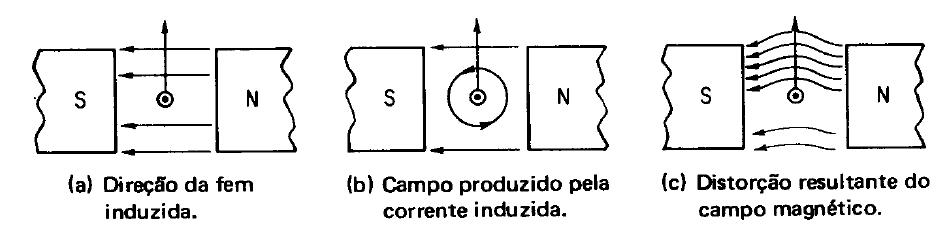
\includegraphics[scale=0.5]{ilustra_lenz}
\caption{Ilustração da lei de Lenz. \cite{kosow}}
\end{figure}
\chapter{Lei de Ampère}
André Marie Ampère estabeleceu uma relação matemática entre corrente elétrica e campo magnético, por meio de uma lei que leva seu nome. Tal pode ser expressada por
\begin{figure}[!ht]
\begin{equation}
\label{enunciado_ampere}
\oint_C \vec{B} dl = \mu_0 i 
\end{equation}
\caption*{Equação \ref{enunciado_ampere}: A lei de Ampère.}
\end{figure}

onde $\mu_0$ é a permeabilidade magnética do espaço livre = $4 \pi \times 10^{-7} H/M$. Ela equivale a dizer que a integral de linha em um caminho fechado da densidade de fluxo, é proporcional à corrente que atravessa a superfície limitada pelo caminho de integração.

\chapter{Força eletro-motriz e força contra-eletro-motriz (FEM, FCEM)}

Seja um transformador com o secundário em aberto sendo alimentado por uma $v_1$ no primário:
\begin{center}
\label{trafo_aberto}
\begin{figure}[htb]

\centering
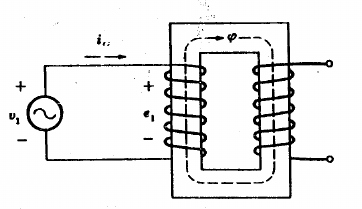
\includegraphics[scale=0.5]{trafo_2_em_aberto}
\caption{Transformador em aberto. \cite{fitzgerald}}
\end{figure}
\end{center}

Em regime permanente, fluirá a corrente de excitação, a qual provoca um fluxo magnético alternado $\phi_1$ no núcleo. Por consequência da lei de Faraday expressa em \ref{enunciado_faraday_integral}, será induzida uma força magnetomotriz nos terminais do secundário, igual a

\begin{equation}
{FEM}_2 = N_2 \frac{d_{\phi 1}}{dt}
\end{equation}

Mas o primário estará sujeito ao fluxo magnético gerado por ele mesmo, e por consequência a uma FEM. Como pela lei de Lenz a polaridade desta FEM será oposta à da sua causa, convencionou chamá-la de \textbf{força contra-eletro-motriz} (FCEM). A soma da FCEM com a queda de tensão no primário deverá ser igual à tensão $v_1$ aplicada, ou seja, $v_1 = R_1 i_\phi + FCEM$.

\chapter{Circuitos Magnéticos}

Circuitos magnéticos são dispositivos utilizados para concentrar o efeito magnético de uma corrente em uma região particular do espaço. Fazendo uma analogia com os circuitos elétricos, temos que \cite{wentworth}: \newline

\begin{center}
\centering

\begin{tabular}{|c|c|c|}
\hline  & Circuito Elétrico & Circuito Magnético. \\ 
\hline Uma fonte de ... & FEM (V) & FMM  (ampère-espira) \\ 
\hline ... produz ... & corrente (A) & fluxo (Wb) \\ 
\hline ... que é limitada pela & resistência ($\Omega$) & relutância ($\frac{1}{H}$)\\ 
\hline 
\end{tabular} 
\end{center}

\begin{center}
\centering
\label{asdf}
\begin{figure}[htb]

\centering
\includegraphics[scale=0.5]{circ_mag}
\caption{Circuito magnético simples com um entreferro (\textit{gap}). \cite{fitzgerald}}
\end{figure}
\end{center}

e em um circuito magnético o fluxo total é calculável por 

\begin{figure}[!ht]
\begin{equation}
\label{def_fluxo}
\Phi = \frac{\mathcal{F}}{\mathcal{R}_{total}}
\end{equation}
\caption*{Equação \ref{def_fluxo}: Relação entre fluxo, FMM (dada por $N i$) e relutância.}
\end{figure}

Define-se relutância em termos da expressão \ref{def_fluxo}, como a oposição do material à passagem do fluxo, isto é, $\mathcal{R} = \frac{FMM}{\Phi}$. Para um material qualquer, esta também pode ser escrita como

\begin{figure}[H]
\begin{equation}
\label{def_relutancia}
\mathcal{R} = \frac{l_c}{\mu A_c}
\end{equation}
\caption*{Equação \ref{def_relutancia}: Definição de relutância para um material de comprimento $l_c$, área $A_c$ e permeabilidade $\mu$.}
\end{figure}

Em muitas situações práticas a relutância do núcleo é desprezível devido ao seu baixíssimo valor perante a relutância do entreferro. No caso do circuito da figura anterior, o cálculo do fluxo ficaria

\begin{figure}[H]
\begin{equation}
\label{relutancia_simples}
\Phi = \frac{N i \mu A_g}{g}
\end{equation}
\caption*{Equação \ref{relutancia_simples}: Fluxo para o circuito magnético mais simples possível.}
\end{figure}

\chapter{Indutância Mútua e Auto-Indutância}

Em um circuito magnético, a relação entre o fluxo $\phi$ e a corrente elétrica \textit{i} geradora será linear, dada pela expressão
\begin{figure}[!ht]
\begin{equation}
\label{def_relacao_fluxo}
L = \frac{\lambda}{i}
\end{equation}
\caption*{Equação \ref{def_relacao_fluxo}: Relação entre o fluxo e corrente elétrica no circuito magnético}
\end{figure}

na qual $\lambda$ é o fluxo concatenado por um conjunto de N espiras ($\lambda = N \phi$). A essa relação dá-se o nome de \textbf{indutância}, expressa em Henries (H).

Presumindo que os materiais magnéticos sejam lineares, pode-se demonstrar (omitido aqui devido à extensão), como feito em \cite{fitzgerald}, que a mesma relação da expressão \ref{def_relacao_fluxo} pode ser expressa em função do número de espiras e da relutância ($\mathcal{R}$), ou seja:

\begin{figure}[!ht]
\begin{equation}
\label{def_relacao_relut}
L = \frac{N^2}{\mathcal{R}}
\end{equation}
\caption*{Equação \ref{def_relacao_relut}: \ref{def_relacao_fluxo} em termos da relutância e do número de espiras.}
\end{figure}

Um caso especial é quando há duas ou mais bobinas no mesmo circuito: temos a auto-indutância (provocada pela variação do campo da própria bobina) de cada bobina e a indutância mútua (provocada na outra bobina pelo campo de uma bobina). Pode-se demonstrar que a indutância entre um par de bobinas X e Y, enroladas em um núcleo de relutância desprezível, será dada por

\begin{figure}
\begin{equation}
\label{ind_mutua_auto}
L_{xy}  = N_x N_y \frac{\mu_0 A_c}{g}
\end{equation}
\caption*{Equação \ref{ind_mutua_auto}: Expressão da indutância entre duas bobinas. Se $X=Y$, ela se refere à autoindutância}
\end{figure}

\chapter{Conclusão}
No presente trabalho foi possível revisar alguns dos conceitos do eletromagnetismo, como as leis de Faraday, Lenz e Ampère, a indutância mútua e os circuitos magnéticos, necessários para o estudo dos transformadores e verificar como eles se aplicam nestes dispositivos. 

\bibliographystyle{alpha}
\begin{thebibliography}{100}
\bibitem{fitzgerald} FITZGERALD, A.E. KINGSLEY, C. Jr. UMANS, S. D. \textbf{Máquinas Elétricas}. 6ª Edição. Porto Alegre: Bookman, 2006.
\bibitem{ulaby} ULABY, F. T. \textbf{Eletromagnetismo para Engenheiros}. Porto Alegre: Bookman, 2006.
\bibitem{kosow} KOSOW, I. L. \textbf{Máquinas Elétricas e Transformadores}. 10ª Edição. São Paulo: Globo, 1994.
\bibitem{assuncao} ASSUNÇÃO, J. T. \textbf{Circuitos Magnéticos}. Disponível em \url{http://www.ppgel.net.br/nepomuceno/ensino/eletromagnetismo/CirMag.pdf}. Acessado em 21/10/2012.
\bibitem{macedo} MACEDO, M. MACEDO. C. \textbf{Indutância}. Disponível em \url{http://www.fisica.ufs.br/apostilas/Fisica_B_Aula_10.PDF}. Acessado em 22/10/2012.
\bibitem{wentworth} WENTWORTH, S. M. \textbf{Eletromagnetismo Aplicado}. Porto Alegre: Bookman, 2007.
\end{thebibliography}
\end{document}          
